\documentclass{article}
\usepackage{booktabs}
\usepackage{tabularx}
\usepackage{float}
\usepackage{graphicx}
\usepackage{geometry}
\geometry{margin=1in}
\begin{document}

\section*{Moda de Evaluaciones en Respuestas a Saludos}

\begin{table}[H]
\centering
\caption{Valor más frecuente por campo}
\begin{tabularx}{0.7\textwidth}{lX}
\toprule
\textbf{Campo} & \textbf{Moda} \\
\midrule
Relevancia & alta \\
Tono & neutral \\
Coherencia_semantica & baja \\
\bottomrule
\end{tabularx}
\end{table}

\begin{figure}[H]
\centering
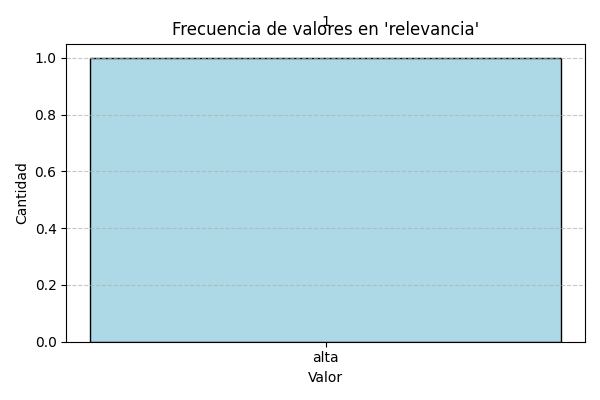
\includegraphics[width=0.8\textwidth]{../graficos/relevancia_frecuencias.png}
\caption{Frecuencia de valores para relevancia}
\end{figure}

\begin{figure}[H]
\centering
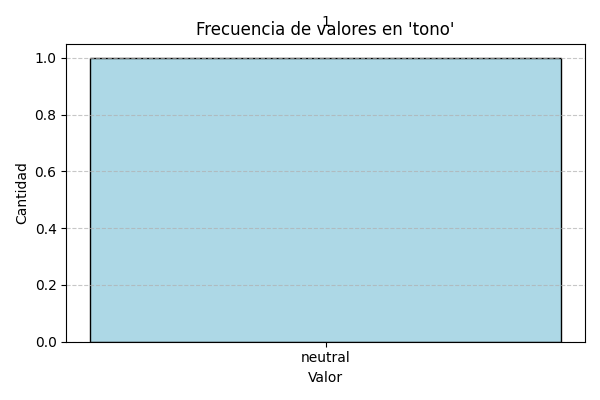
\includegraphics[width=0.8\textwidth]{../graficos/tono_frecuencias.png}
\caption{Frecuencia de valores para tono}
\end{figure}

\begin{figure}[H]
\centering
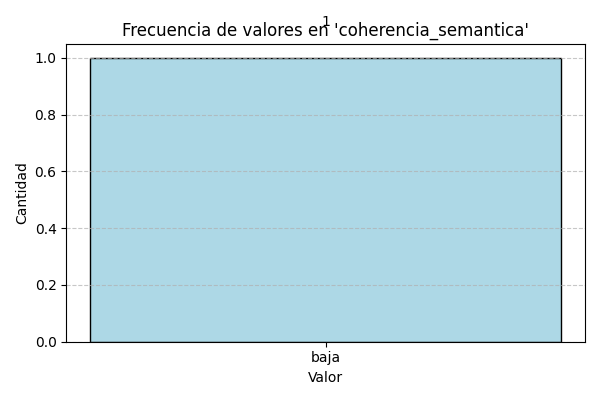
\includegraphics[width=0.8\textwidth]{../graficos/coherencia_semantica_frecuencias.png}
\caption{Frecuencia de valores para coherencia semantica}
\end{figure}
\end{document}